\chapter{Kiến thức nền tảng}
\label{Chapter2}

\textit{Trong chương này, chúng tôi trình bày các kiến thức nền tảng được sử dụng trong khóa luận. Đầu tiên, chúng tôi giới thiệu tổng quan về mạng nơ-ron nhiều tầng ẩn cũng như quá trình huấn luyện một mô hình mạng nơ-ron và những khó khăn cần khắc phục. Tiếp theo chúng tôi giới thiệu thuật toán tối ưu Gradient Descent và hai phiên bản của thuật toán đó là ``Batch Gradient Descent'' (BGD) và ``Minibatch Gradient Descent'' (MGD) là nền tảng cho các thuật toán tối ưu sau này nhằm giải quyết các khó khăn trong huấn luyện mạng nơ-ron.}

\section{Mạng nơ-ron nhiều tầng ẩn}

Ngay từ những ngày đầu tiên của điện toán, những nhà khoa học đã hướng đến việc tạo ra những chiếc máy tính có thể thực hiện các tác vụ đòi hỏi khả năng suy nghĩ như bộ não con người. Mục tiêu cuối cùng của những chiếc máy tính này là thay thế con người thực hiện các tác vụ phức tạp như nhận diện vật thể trong hình ảnh, hiểu được ý nghĩa của ngôn ngữ tự nhiên, cũng như chơi được những trò chơi trí tuệ như cờ vua và cờ vây. Hướng nghiên cứu những phương pháp cung cấp cho máy tính khả năng suy nghĩ như con người được gọi là ``trí tuệ nhân tạo'' (artificial intelligence).

Các phương pháp trí tuệ nhân tạo truyền thống có thể giải quyết được một số bài toán như tìm đường đi tối ưu một cách nhanh hơn, giải một số trò chơi như 8-puzzle, và thậm chí có thể đánh cờ vua ở trình độ Grandmaster (Đại kiện tướng)\cite{campbell2001deepblue}. Tuy nhiên, những phương pháp này chưa đủ sức tự giải quyết được các bài toán cấp cao hơn như nhận diện thông tin trong ảnh và văn bản. Lí do là vì trí tuệ nhân tạo truyền thống cần con người tạo ra các ``đặc trưng thủ công'' (hand-crafted features) dựa trên những hiểu biết của con người về dữ liệu và bài toán đó. Một hướng nghiên cứu hướng tới việc máy tính có thể tự học và rút trích những đặc trưng đó một cách tự động thông qua việc huấn luyện một mô hình thích ứng với dữ liệu được gọi là ``học máy'' (machine learning). Các mô hình học máy cho phép máy tính có thể chuyển đổi các đặc trưng đơn giản ban đầu thành ``kiến thức'' để hỗ trợ trong việc dự đoán. Nhờ có những kiến thức này mà các mô hình học máy có thể dùng để ứng dụng trong nhiều lĩnh vực khác nhau.

\begin{figure}[htp]
\centering
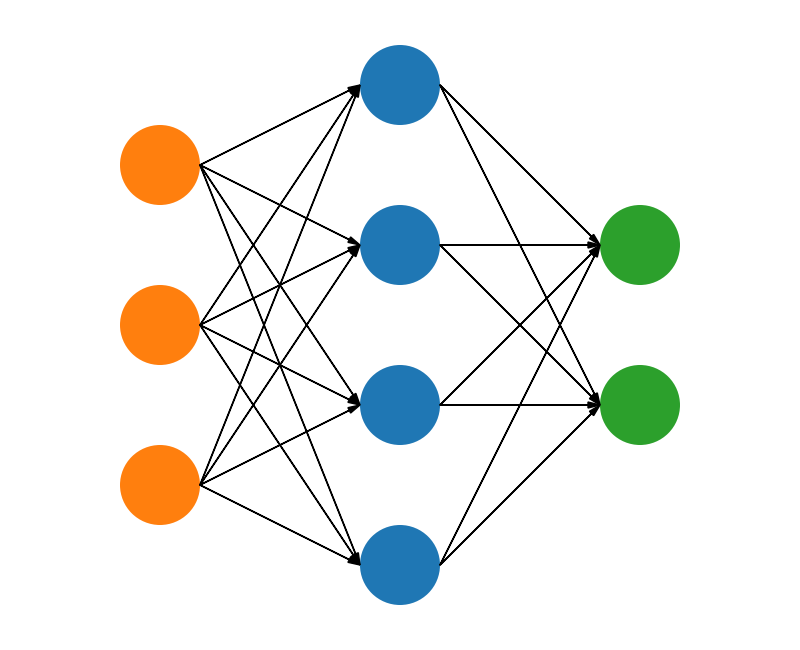
\includegraphics[width=80 mm]{images/ann.png}
\caption{Mô hình mạng nơ-ron nhân tạo với tầng nhập (màu cam), tầng ẩn (màu xanh dương) và tầng xuất (màu xanh lá).}
\label{fig:ann}
\end{figure}

Trong số những phương pháp học máy được phát triển, một nhóm phương pháp tên là mạng nơ-ron nhân tạo (artificial neural network) (Hình \ref{fig:ann}) cố gắng mô phỏng lại cách các nơ-ron thần kinh trong não người liên kết với nhau để xử lý tín hiệu đầu vào từ các giác quan và truyền tín hiệu đã qua xử lý cho các nơ-ron tiếp theo. Sự đòi hỏi lớn về đơn vị tính toán là khó khăn khiến cho các thuật toán học máy truyền thống không thể giải quyết tốt các bài toán mà hàm số biểu diễn chúng phụ thuộc vào nhiều biến số biểu diễn tốt các hàm này. Thêm nữa, các thuật toán học máy truyền thống không hoạt động tốt đối với những dữ liệu mới, nên việc ứng dụng các mô hình này vào thực tế bị hạn chế. Mạng nơ-ron cho phép kết hợp nhiều hàm phức tạp bằng các nơ-ron được liên kết với nhau. Sự kết hợp này cho phép thực hiện những dự đoán vừa phụ thuộc vào dữ liệu huấn luyện vừa có thể tự tổng quát hoá cho dữ liệu mới.

Trong môi trường máy tính, mỗi ``nơ-ron'' nhân tạo là một hàm số ánh xạ các tín hiệu đầu vào tới một tín hiệu đầu ra (Hình \ref{fig:perceptron-node}). Mỗi tín hiệu đầu vào sẽ được nhân với trọng số tương ứng. Tổng của các tín hiệu này sẽ được cộng với một hệ số bias riêng biệt của tầng nơ-ron đó trước khi đi qua một ``hàm kích hoạt'' (activation function). Hàm kích hoạt đóng vai trò quyết định việc tín hiệu sẽ được biến đổi như thế nào sau khi đi qua nơ-ron đó.

\begin{figure}[htp]
\centering
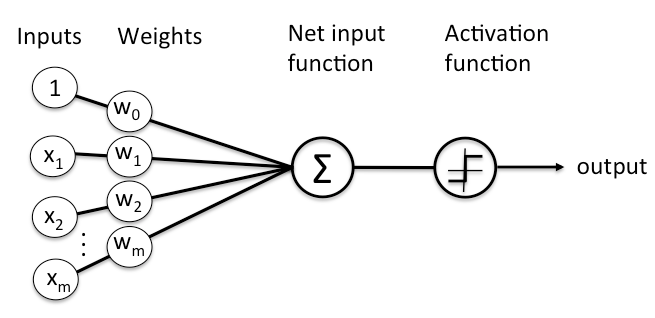
\includegraphics[width=120 mm]{images/perceptron-node.png}
\caption{Minh họa cách hoạt động của một nơ-ron. (Nguồn: \url{https://wiki.pathmind.com/neural-network})}
\label{fig:perceptron-node}
\end{figure}

Một hàm số càng có nhiều biến số sẽ càng cần nhiều nơ-ron để biểu diễn lại hàm số đó, đồng nghĩa với việc cần một lượng dữ liệu rất lớn để ``học'' được hàm số đó. Sử dụng mạng nơ-ron nhiều tầng ẩn giúp biểu diễn một hàm số có độ phức tạp tương đương nhưng với số lượng nơ-ron ít hơn rất nhiều, theo đó là số lượng dữ liệu cần để huấn luyện cũng giảm đi đáng kể\cite{bengio2007scaling}.

``Mạng nơ-ron nhiều tầng ẩn'' (deep neural network) mở rộng mô hình theo chiều sâu, tăng số lượng tầng ẩn trung gian thay vì tăng số lượng nơ-ron cho một tầng ẩn duy nhất. Hình \ref{fig:dnn} mô tả một mạng nơ-ron nhiều tầng ẩn đơn giản với một tầng nhập, hai tầng ẩn và một tầng xuất.

\begin{figure}[H]
\centering
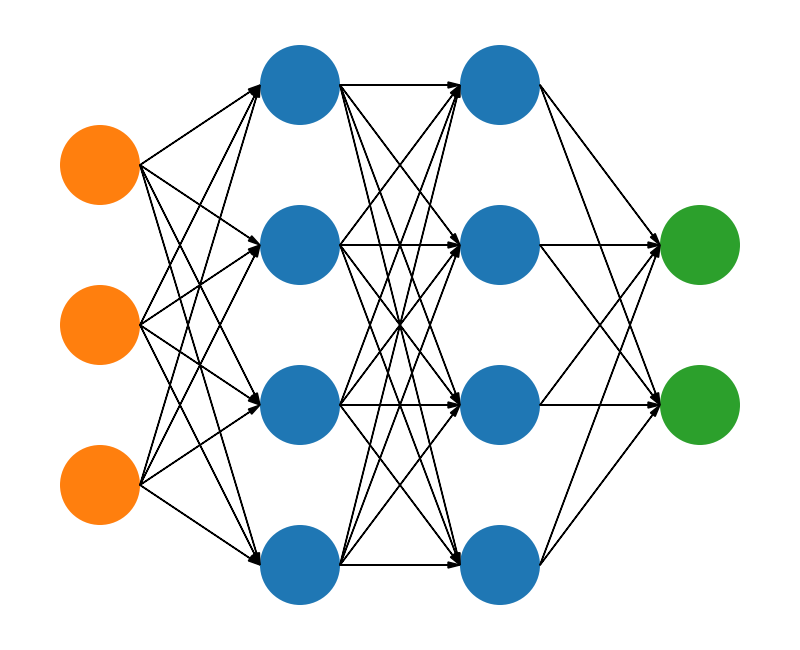
\includegraphics[width=80 mm]{images/dnn.png}
\caption{Mô hình mạng nơ-ron nhiều tầng ẩn với tầng nhập (màu cam), các tầng ẩn (màu xanh dương) và tầng xuất (màu xanh lá)}
\label{fig:dnn}
\end{figure}

Quá trình truyền thẳng dữ liệu qua mạng no-ron nhiều tầng ẩn cũng có thể được biểu diễn dưới dạng các hàm số được xâu chuỗi với nhau. Xét mạng nơ-ron có 2 tầng ẩn ở Hình \ref{fig:dnn}, chúng ta có thể biểu diễn mô hình đó bằng công thức $\hat{y}=f^{(2)}(f^{(1)}(x))$ với $f^{(1)}$ là tầng ẩn thứ nhất và $f^{(2)}$ là tầng ẩn thứ 2, và $\hat{y}$ sẽ là giá trị cuối cùng mà mô hình dự đoán được từ dữ liệu đầu vào $x$. Qua mỗi hàm $f^{(i)}$ trung gian, dữ liệu của tầng trước sẽ bị biến đổi phi tuyến, hay ánh xạ dữ liệu sang chiều không gian khác, và truyền đến tầng tiếp theo.

\begin{figure}[H]
\centering
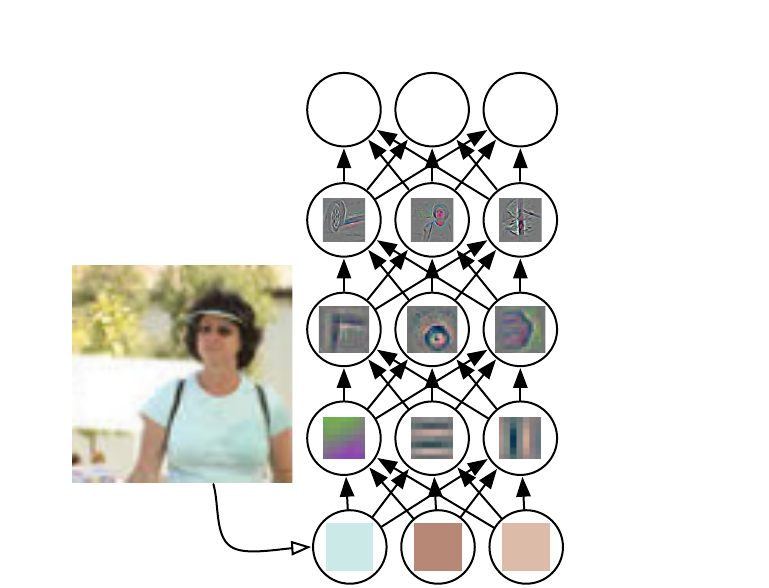
\includegraphics[width=80 mm]{images/dnn-features.png}
\caption{Quá trình mạng nơ-ron trích xuất các đặc trưng của dữ liệu\cite{goodfellow2016deeplearning}.}
\label{fig:dnn-features}
\end{figure}

Ngoài trích xuất được thêm thông tin, các tầng ẩn còn có khả năng kết hợp các đặc trưng đơn giản ở tầng trước đó thành các đặc trưng cấp cao hơn. Hình \ref{fig:dnn-features} cho thấy ở tầng ẩn đầu tiên, mô hình kết hợp các giá trị điểm ảnh thành các đường nét đơn giản. Sau đó ở tầng tiếp theo, các đường nét được kết hợp thành các hình dạng. Từ các hình dạng, mạng nơ-ron hình thành những vật thể hoàn chỉnh hơn và đưa ra dự đoán. Như vậy, chúng ta có thể thấy được rằng, với càng nhiều tầng ẩn, mô hình mạng nơ-ron sẽ càng rút trích thông tin tốt hơn, từ đó tăng cường khả năng xử lý các bài toán phức tạp.

\section{Quá trình huấn huyện mạng nơ-ron nhiều tầng ẩn}

Xét một bài toán học có giám sát (supervised learning), chúng ta có tập dữ liệu huấn luyện $X$ và tập giá trị đúng (ground truth) $Y$. Mô hình mạng nơ-ron là một hàm $\mathcal{F}: (\theta, x) \rightarrow \hat{y}$ với $x$ là một điểm dữ liệu và $\hat{y}$ là giá trị mà mạng nơ-ron dự đoán ra dựa theo bộ trọng số $\theta$. Như vậy, với tập dữ liệu huấn luyện $X$ và tập giá trị đúng $Y$, chúng ta sẽ tính được độ lỗi của mô hình trên toàn tập dữ liệu huấn luyện với một hàm chi phí $\mathcal{L}(\theta)$ với $\theta$ là bộ trọng số của mô hình mạng nơ-ron:

\begin{equation}
\label{eqn:E-y}
\mathbf{\it{E}(\theta)} = \frac{1}{N}\cdot \sum_{i=1}^{N}\mathcal{L}(\hat{y_i}, y_i)
\end{equation}
\begin{equation}
\label{eqn:E-Fx}
\\\Rightarrow \mathbf{\it{E}(\theta)} = \frac{1}{N}\cdot \sum_{i=1}^{N}\mathcal{L}(\mathcal{F}_\theta( x_i), y_i)
\end{equation}

Trong đó, $\theta$ là bộ trọng số của mô hình, $x_i = \{x_1, x_2,...x_N\}$ là tập các tín hiệu đầu vào và $N$ là kích thước tập dữ liệu huấn luyện, hàm $\mathcal{L}(\mathcal{F}_\theta( x_i), y_i)$ là hàm đánh giá độ lỗi của mạng nơ-ron với bộ trọng số $\theta$ và điểm dữ liệu $x_i$. Trung bình của các độ lỗi này là hàm chi phí $E(\theta)$ mà ta cần tối ưu. Với hàm chi phí $E(\theta)$ và không gian cao chiều được tạo bởi bộ trọng số, ta được một bề mặt phẳng lỗi $M$ chiều với $M$ là số trọng số của mạng nơ-ron.

Vì vậy, ta có thể đưa quá trình huấn luyện mạng nơ-ron thành quá trình đi tìm vị trí mà tại đó hàm chi phí $E(\theta)$ đạt giá trị cực tiểu. Giá trị cực tiểu này phải có độ lỗi rất nhỏ trên tập huấn luyện, đồng thời phải có độ lỗi đủ nhỏ trên dữ liệu ngoài tập huấn luyện để đảm bảo tính tổng quát hóa của mô hình. Tuy nhiên, việc đi tìm giá trị cực tiểu này gặp nhiều khó khăn do bộ trọng số của mô hình mạng nơ-ron nhiều tầng ẩn có số chiều rất lớn, cách giải phương trình thông thường không thể áp dụng tốt trong trường hợp này. Hơn nữa, mỗi trọng số có mức độ ảnh hưởng khác nhau lên độ lỗi làm xuất hiện các điểm cực tiểu địa phương và điểm yên ngựa, các vùng bằng phẳng hay các vùng rãnh hẹp phức tạp.

``Critical point'' (điểm tới hạn) là điểm mà tại đó hàm số không khả vi hoặc có đạo hàm bằng 0. Theo đó, cực tiểu địa phương của một hàm $f(x)$ là một điểm cực trị a trong một khoảng xác định có giá trị $f(a)$ không lớn hơn bất kỳ giá trị $f(x)$ với mọi $x$ trong khoảng đó (Hình \ref{fig:minimas}a). Công trình của D. Erhan và cộng sự\cite{erhan2009thedifficulty} đã chứng minh rằng mạng nơ-ron nhiều tầng ẩn rất dễ hội tụ tại các điểm cực tiểu có độ lỗi khá cao nếu khởi tạo ngẫu nhiên. Các điểm này từng được coi là vấn đề chính trong việc hạn chế độ chính xác của mô hình và gây trở ngại trong việc ứng dụng các mô hình mạng nơ-ron nhiều tầng ẩn vào thực tế. Tuy nhiên một số nghiên cứu gần đây cho rằng điểm cực tiểu địa phương không phải là khó khăn chính cản trở quá trình huấn luyện của mạng nơ-ron nhiều tầng ẩn mà chính các điểm yên ngựa mới là trở ngại cho các thuật toán tối ưu\cite{dauphin2014identifying}.

\begin{figure}[htp]
\centering
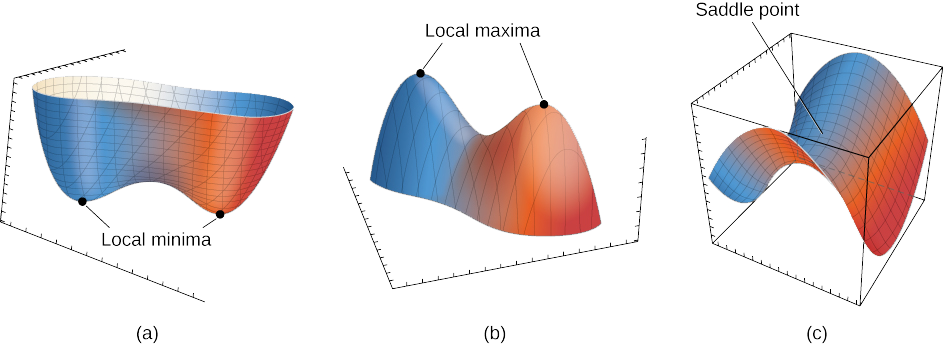
\includegraphics[width=120 mm]{images/minimas.png}
\caption{Minh hoạ điểm cực tiểu (a), cực đại (b) và điểm yên ngựa (c) trong không gian ba chiều.}
\label{fig:minimas}
\end{figure}

Một hàm số $f(x,y)$ có điểm dừng tại $(a,b)$ nhưng tại đó hàm số $f(x,y)$ không có cực trị, ta gọi điểm $(a,b)$ là điểm yên ngựa (Hình \ref{fig:minimas}c). Trong các mạng nơ-ron nông, điểm yên ngựa chiếm tỉ lệ rất ít trong số các critical point, đa số các critical point được tìm thấy là các cực tiểu địa phương. Tuy nhiên, Yann N. Dauphin đã chỉ ra rằng khi số lượng tầng ẩn trong mạng càng tăng thì tỉ lệ xuất hiện của các điểm yên ngựa là càng cao và gần như tất cả các critical point được tìm thấy là điểm yên ngựa có độ lỗi cao hơn rất nhiều độ lỗi của cực tiểu toàn cục \cite{dauphin2014identifying}. Đồng thời, bài báo cũng chỉ ra rằng trong không gian cao chiều, xác suất để tất cả các hướng xung quanh một critical point có đường cong lên là rất thấp, nghĩa là tần suất xuất hiện của cực tiểu địa phương là rất nhỏ. Vì những lý do trên mà các yên ngựa được coi là lý do lớn gây cản trở quá trình tối ưu mạng nơ-ron nhiều tầng ẩn.

Có hai khó khăn chính cần phải giải quyết khi gặp điểm yên ngựa: (1) Tìm được hướng có đường cong hướng xuống trong mặt phẳng lỗi để tiến tới điểm có độ lỗi nhỏ hơn, và (2) vượt qua vùng bằng phẳng, là vùng có độ dốc gần như bằng nhau, bao bọc xung quanh điểm yên ngựa. Trong các thuật toán tối ưu sử dụng đạo hàm bậc nhất, mặc dù hướng gradient trùng với hướng có đường cong hướng xuống trong mặt phẳng lỗi và có thể hướng tới điểm có độ lỗi nhỏ hơn, nhưng các bước cập nhật diễn ra rất chậm do độ dốc của các điểm này rất nhỏ và dường như bằng nhau trong vùng lân cận. Để khắc phục được khó khăn này, một số thuật toán bậc nhất đã cố gắng xấp xỉ thông tin đạo hàm bậc hai để có thêm thông tin về độ cong của mặt phẳng lỗi tại điểm đang xét. Các thuật toán này đều là những cải tiến của thuật toán Gradient Descent.

\section{``Gradient Descent''}

\begin{figure}[H]
\centering
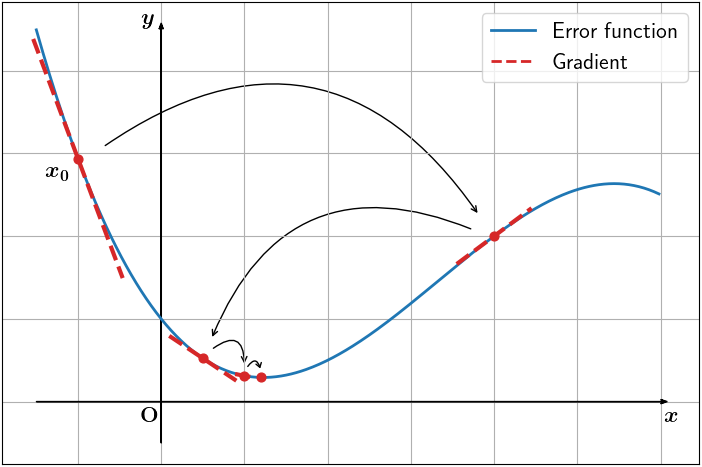
\includegraphics[width=75 mm]{images/gd.png}
\caption{Minh họa quá trình tìm đến điểm cực tiểu của thuật toán Gradient Descent với đường màu xannh dương biểu diễn giá trị của hàm chi phí, đường đứt đoạn màu đỏ thể hiện phương và độ lớn của gradient.}
\label{fig:gd}
\end{figure}

``Gradient Descent'' là thuật toán cho phép đi tìm cực tiểu của một hàm số mà không cần biết chính xác công thức của hàm số đó bằng cách di chuyển từng bước nhỏ cho đến khi hội tụ tại cực tiểu (Hình \ref{fig:gd}). Bằng cách sử dụng khai triển Taylor, ta có thể xấp xỉ đạo hàm bậc k của bất kỳ hàm số nào, cho phép Gradient Descent giải quyết được hầu hết các hàm số được dùng trong huấn luyện mạng nơ-ron nhiều tầng ẩn.

\begin{itemize}
	\item Khai triển Taylor: Công thức \ref{eqn:taylor-f} cho xấp xỉ đạo hàm bậc $k$ của một hàm số $f(x)$ quanh một điểm $x$ với $\Delta x$ đủ nhỏ.
	\begin{equation} \label{eqn:taylor-f}
		f(x + \Delta x) \approx f(x) + f'(x)\Delta x + \frac{1}{2!}f''(x)(\Delta x)^2 +...+ \frac{1}{k!}f^{(k)} (\Delta x)^{(k)}
	\end{equation}
	Từ đó, để có thể cực tiểu hóa hàm chi phí $\mathcal{L}$, Gradient Descent sẽ di chuyển theo hướng $\Delta x$ sao cho $\mathcal{L}(x + \Delta x) < \mathcal{L}(x)$ và bằng:
	\begin{equation} \label{eqn:l_x-delta}
	\mathcal{L}(x + \Delta x) \approx \mathcal{L}(x) + \Delta x\nabla_x \mathcal{L}
	\end{equation}
	với $\nabla_x\mathcal{L}$ là gradient của hàm chi phí $\mathcal{L}$ tại $x$.

	\item Gradient là véc-tơ có hướng là hướng có mức độ tăng lớn nhất và độ lớn là mức độ thay đổi lớn nhất tại một điểm trong không gian. Giả sử một không gian $\mathbb{R}^n$ được định nghĩa bởi một hàm $f(x_1,x_2,x_3,...,x_n)$ thì véc-tơ gradient tại một điểm trong không gian $\mathbb{R}^n$ sẽ là một véc-tơ cột mà thành phần của nó là đạo hàm theo từng biến của hàm $f(x_1,x_2,x_3,...,x_n)$, cụ thể là:
	\begin{equation} \label{eqn:grad_f}
	\nabla f = (\frac{\delta f}{\delta x_1}, \frac{\delta f}{\delta x_2}, \frac{\delta f}{\delta x_3},...,\frac{\delta f}{x_n})
	\end{equation}
\end{itemize}

Vì gradient chỉ hướng có mức độ tăng lớn nhất nên hướng $\Delta x$ cho giá trị của $\mathcal{L} (x + \Delta x)$ giảm nhiều nhất theo hướng $-\nabla_x\mathcal{L}$. Tuy nhiên, $\Delta x$ phải có giá trị đủ nhỏ để xấp xỉ Taylor vẫn đảm bảo rằng hướng $\Delta x$ sẽ cho giá trị $\mathcal{L}(x + \Delta x) < \mathcal{L}(x)$. Từ đó, ta áp dụng một hằng số dương $\eta$ đảm bảo độ dài của một bước đi $\Delta x$ đủ nhỏ, được gọi là tỷ lệ học (learning rate). Vậy ta có thể viết được công thức cập nhật của Gradient Descent tại mỗi bước nhảy $x_t$ như sau:

\begin{equation} \label{eqn:L_x-delta}
\mathcal{L}(x_t + \Delta x) \approx \mathcal{L}(x_t) - \eta{(\nabla_{x_t} \mathcal{L})^T\nabla _{x_t}\mathcal{L}}
\end{equation}
Lại có: $(\nabla _{x_t}\mathcal{L})^T\nabla _{x_t} \mathcal{L} > 0 \Rightarrow \mathcal{L}(x_t + \Delta x) < \mathcal{L}(x_t)$.

Với hằng số $\eta$ cố định công thức \ref{eqn:l_x-delta} sẽ luôn tiến hành cập nhật một lượng $\Delta x = \eta (\nabla _{x_t}\mathcal{L})^T\nabla _{x_t}\mathcal{L} = \eta ||\nabla _{x_t}\mathcal{L}||_2$ thay đổi tương ứng tỷ lệ với $||\nabla _{x_t} \mathcal{L}||_2$. Nếu $||\nabla _{x_t} \mathcal{L}||_2$ lớn, có nghĩa là độ dốc lớn, ta có thể bước một bước dài để tiến nhanh tới giá trị cực tiểu. Ngược lại, nếu $||\nabla_{x_t} \mathcal{L}||_2$ nhỏ, độ dốc nhỏ, ta phải bước những bước nhỏ để tránh bị vượt qua khỏi vùng cực tiểu.

Bên cạnh đó, nếu tỷ lệ học quá nhỏ, ta luôn bước những bước rất nhỏ hướng về phía cực tiểu nên sẽ mất rất nhiều thời gian để thuật toán có thể hội tụ. Tuy nhiên, nếu chọn một tỷ lệ học quá lớn thì xấp xỉ Taylor không đảm bảo được rằng giá trị $\mathcal{L}(x + \Delta x)$ sẽ giảm và thuật toán có khả năng không thể hội tụ. Đó là lý do tại sao lựa chọn một tỷ lệ học phù hợp là cần thiết.

\subsection{``Batch'' Gradient Descent}

Thuật toán ``Batch Gradient Descent'' (BGD) là một phiên bản của thuật toán Gradient Descent sử dụng gradient của toàn bộ dữ liệu huấn luyện để thực hiện một bước cập nhật. Vì độ lỗi được tính tại các điểm dữ liệu riêng lẻ, nên trung bình các độ lỗi này sẽ là độ lỗi của cả tập dữ liệu (Công thức \ref{eqn:E-Fx}).

Từ công thức \ref{eqn:L_x-delta} và (9), ta có thể viết được công thức cập nhật của $\theta$ tại mỗi bước:

\begin{equation}
\theta_{t+1} = \theta_ t - \eta \nabla_{\theta} \mathbf{\it{E}(\theta)}
\end{equation}
với $\nabla_\theta \mathbf{\it{E}(\theta)}$ là gradient của hàm chi phí được tính trên toàn tập dữ liệu.

Tổng quan thuật toán BGD được trình bày trong thuật toán \ref{alg:BGD}.

\begin{algorithm}
	\caption{Batch Gradient Descent (BGD)} \label{alg:BGD}
	\begin{algorithmic}[1]
		\renewcommand{\algorithmicrequire}{\textbf{Đầu vào:}}
		\renewcommand{\algorithmicensure}{\textbf{Đầu ra:}}
		\algnewcommand\algorithmicoperation{\textbf{Thao tác:}}
		\algnewcommand\Operation{\item[\algorithmicoperation]}

		\Require Tập dữ liệu huấn luyện $x_i (i = 1, 2, ..., N)$, tỉ lệ học $\eta$, bộ trọng số $\theta$ của mô hình $\mathcal{F}$
		\Ensure Bộ trọng số $\theta$ của $\mathcal{F}$ với độ lỗi đạt cực tiểu

		\Operation
		\While{$\theta$ chưa hội tụ}
			\State Tính độ lỗi trung bình: $\mathbf{\it{E}(\theta)} \gets \frac{1}{N}\cdot \displaystyle\sum_{i=1}^{N}\mathcal{L}(\hat{y_i}, y_i)$
			\State Thực hiện cập nhật trọng số: $\theta \gets \theta - \eta \nabla_{\theta} \mathbf{\it{E}(\theta)}$
		\EndWhile
		\State return $\theta$
	\end{algorithmic}
\end{algorithm}

\subsection{``Minibatch'' Gradient Descent}

Một trong những trở ngại của BGD khi ứng dụng vào việc huấn luyện mạng nơ-ron nhiều tầng ẩn là tốc độ huấn luyện. Việc huấn luyện một mạng nơ-ron nhiều tầng ẩn thường đòi hỏi một tập dữ liệu rất lớn để mô hình có thể học đủ thông tin về các đặc trưng của dữ liệu. Trong mỗi bước, BGD cần duyệt qua từng điểm dữ liệu trong tập dữ liệu huấn luyện, tính độ lỗi và véc-tơ đạo hàm riêng của độ lỗi theo từng trọng số, cuối cùng là tính trung bình của các véc-tơ đạo hàm để có được véc-tơ gradient $\nabla_{\theta}\mathbf{\it{E}}(\theta)$, và chúng ta chỉ dùng một phần nhỏ của độ dài gradient đó để cập nhật.

Có thể thấy BGD mất rất nhiều thời gian để duyệt qua hết toàn bộ tập dữ liệu, nhưng chỉ cải thiện được một lượng rất nhỏ. Để khắc phục nhược điểm này, ``Minibatch Gradient Descent'' (MGD) chỉ thực hiện tính gradient của hàm chi phí trên một tập con của tập dữ liệu (thường gọi là một ``minibatch'') để thực hiện một bước cập nhật.

Từ công thức (6) và (7) của BGD, chúng ta sẽ có công thức tính độ lỗi của MGD với một tập con:

\begin{equation}
\label{eqn:E-minibatch}
\mathbf{\it{E}(\theta)} = \frac{1}{k}\cdot \sum_{i=1}^{k}\mathcal{L}(\mathcal{F}_\theta( x_i), y_i)
\end{equation}
với $k$ là kích thước của một tập con ($k<<N$). Từ độ lỗi tính được, việc cập nhật trọng số cho mạng nơ-ron nhiều tầng ẩn được thực hiện tương tự như BGD bằng công thức (7).

Như vậy, có thể thấy được rằng một bước cập nhật với MGD sẽ nhanh hơn rất nhiều so với BGD do việc tính toán chỉ thực hiện trên $k$ điểm dữ liệu và cập nhật theo gradient của tập con đó. Ngoài ra, trong mỗi lần duyệt qua toàn bộ tập dữ liệu (gọi là một ``epoch''), MGD thực hiện được $N/k$ lần cập nhật trọng số cho mô hình, thay vì chỉ một lân như BGD. Điều đó cũng đồng nghĩa rằng với cùng một số lượng epoch huấn luyện, MGD sẽ đi được rất nhiều bước so với BGD.

Một trường hợp đặc biệt của MGD là khi $k=1$, được gọi là ``Stochastic Gradient Descent'' (SGD). Tuy nhiên hiện nay khi nhắc đến SGD trong bài toán tối ưu mạng nơ-ron nhiều tầng ẩn, người ta thường ám chỉ MGD với $k>1$, từ ``Stochastic'' ám chỉ cách chọn các tập con từ tập dữ liệu huấn luyện là ngẫu nhiên. Việc sử dụng khái niệm ``Batch'' trong BGD cũng dễ gây nhầm lẫn vì từ ``Batch'' mang ý nghĩa một tập hợp của thứ gì đó, như ``batch size'' là kích thước của một tập con, nhưng ở đây lại ám chỉ cả tập dữ liệu huấn luyện\cite{goodfellow2016deeplearning}.

Trong đa số các bài báo khoa học, các tác giả sử dụng khái niệm ``Gradient Descent'' (GD) để chỉ BGD, và ``Stochastic Gradient Descent'' để nói tới MGD. Để tạo sự thống nhất cũng như thuận tiện trong việc liên hệ giữa nội dung khoa luận với nội dung của các bài báo khoa học, từ thời điểm này, chúng tôi cũng sẽ sử dụng cách gọi tên tương tự cho các thuật toán này.

Việc chỉ sử dụng một tập con của dữ liệu huấn luyện để tính gradient cũng đồng nghĩa với việc hướng của gradient này sẽ chỉ xấp xỉ gradient tính được trên cả tập dữ liệu (có thể gọi là ``true gradient''), và sẽ có những sự dao động. Tuy nhiên, nhiều nghiên cứu đã chỉ ra rằng các véc-tơ gradient của các tập con sẽ dao động xung quanh hướng của véc-tơ gradient tính được theo GD với độ chênh lệch không quá lớn\cite{bottou2010large}\cite{bottou2018optimization}. Việc lựa chọn kích thước tập con $k$ là sự đánh đổi giữa mức độ dao động với tốc độ tính toán cũng như số bước cập hật được thực hiện trong mỗi epoch. Khi $k$ tiến tới gần $N$, hướng gradient của tập con sẽ xấp xỉ hướng của true gradient tốt hơn, nhưng lại mất nhiều thời gian tính toán hơn. Ngược lại, khi $k$ tiến gần về 1, tuy thời gian tính toán được rút ngắn nhưng hướng gradient của tập con càng chênh lệch nhiều so với hướng của true gradient, gây ra sự nhiễu loạn.

Tổng quan thuật toán SGD được trình bày trong thuật toán \ref{alg:SGD}.

\begin{algorithm}
	\caption{Batch Gradient Descent (BGD)} \label{alg:SGD}
	\begin{algorithmic}[1]
		\renewcommand{\algorithmicrequire}{\textbf{Đầu vào:}}
		\renewcommand{\algorithmicensure}{\textbf{Đầu ra:}}
		\algnewcommand\algorithmicoperation{\textbf{Thao tác:}}
		\algnewcommand\Operation{\item[\algorithmicoperation]}

		\Require Tập dữ liệu huấn luyện $x_i (i = 1, 2, ..., N)$, kích thước tập con $k$, tỉ lệ học $\eta$, bộ trọng số $\theta$ của mô hình $\mathcal{F}$
		\Ensure Bộ trọng số $\theta$ của $\mathcal{F}$ với độ lỗi đạt cực tiểu

		\Operation
		\While{$\theta$ chưa hội tụ}
			\State Xáo trộn tập dữ liệu.
			\For{mỗi tập con kích thước $k$}
				\State Tính độ lỗi trung bình: $\mathbf{\it{E}(\theta)} \gets \frac{1}{k}\cdot \displaystyle\sum_{i=1}^{k}\mathcal{L}(\hat{y_i}, y_i)$
				\State Thực hiện cập nhật trọng số: $\theta$ $\gets$ $\theta - \eta \nabla_{\theta} \mathbf{\it{E}(\theta)}$
			\EndFor
		\EndWhile
		\State return $\theta$
	\end{algorithmic}
\end{algorithm}

\section{``Lan truyền ngược'' (Backpropagation)}

Quá trình huấn luyện mạng nơ-ron cần tìm một bộ trọng số cho độ lỗi là nhỏ nhất và việc tìm kiếm này có thể được hoàn thành bằng các thuật toán tối ưu đã trình bày ở trên. Tuy nhiên các thuật toán tối ưu này cần véc-tơ đạo hàm riêng của hàm chi phí tại từng trọng số, có nghĩa là ta muốn tìm sự phụ thuộc của độ lỗi và các giá trị trọng số trong mạng. Thuật toán lan truyền ngược có thể giải quyết được vấn đề này bằng cách ``lan truyền'' độ lỗi trở lại trong mạng, từ đó có thể thay đổi giá trị của các trọng số tương ứng với mức độ ảnh hưởng lên độ lỗi. Ý tưởng cho thuật toán được giới thiệu trong bài báo của nhóm tác giả David Rumelhart, Geoffrey Hinton và Ronald Williams dưới cái tên Generalized Delta Rule\cite{rumelhart1986learning}. Thuật toán ra đời đã đánh dấu một sự phát triển vượt bậc trong việc huấn luyện mạng nơ-ron nhiều tầng ẩn và nhận được sự quan tâm rất lớn trong cộng đồng nghiên cứu.

Thuật toán lan truyền ngược là một phép vi phân ngược (reverse-mode differentiation) sử dụng quy tắc mắt xích (chain rule) để tính toán mức độ ảnh hưởng của một trọng số lên giá trị độ lỗi của mạng nơ-ron nhiều tầng ẩn và được thể hiện qua giá trị độ lớn của các phần tử trong véc-tơ $\nabla_\theta \mathbf{\it{E}(\theta)}$ tương ứng cho từng trọng số. Nếu một phần tử trong véc-tơ $\nabla_\theta \mathbf{\it{E}(\theta)}$ có giá trị lớn, nghĩa là khi thay đổi trọng số tương ứng một lượng nhỏ thì độ lỗi sẽ thay đổi một lượng lớn, và ngược lại, nếu một phần tử trong $\nabla_\theta \mathbf{\it{E}(\theta)}$ có giá trị nhỏ bị thay đổi thì độ lỗi sẽ chỉ biên thiên một lượng nhỏ. Vì tính chất đó mà ta gọi giá trị này là ``độ nhạy cảm'' của trọng số.

``Độ nhạy cảm'' của một trọng số $w_i \in \theta$ được tính bằng tỉ lệ giữa độ biến thiên của trọng số đó và độ biến thiên của hàm chi phí $\mathbf{\it{E}(\theta)}$ và bằng đạo hàm riêng của hàm $\mathbf{\it{E}(\theta)}$ tại từng trọng số: $\frac{\delta E}{\delta w_1}; \frac{\delta E}{\delta w_2};...;\frac{\delta E}{\delta w_n}$. Tổng hợp của các giá trị này cho ta véc-tơ $\nabla_\theta \mathbf{\it{E}(\theta)}$. Để dễ dàng trong việc giải thích cách thuật toán thực thi, ta sử dụng một mạng nơ-ron nhiều tầng ẩn đơn giản, được mô tả như Hình \ref{fig:wandb} với 1 tầng nhập, 2 tầng ẩn và 1 tầng xuất, mỗi tầng chỉ có một nơ-ron.

\begin{figure}[htp]
\centering
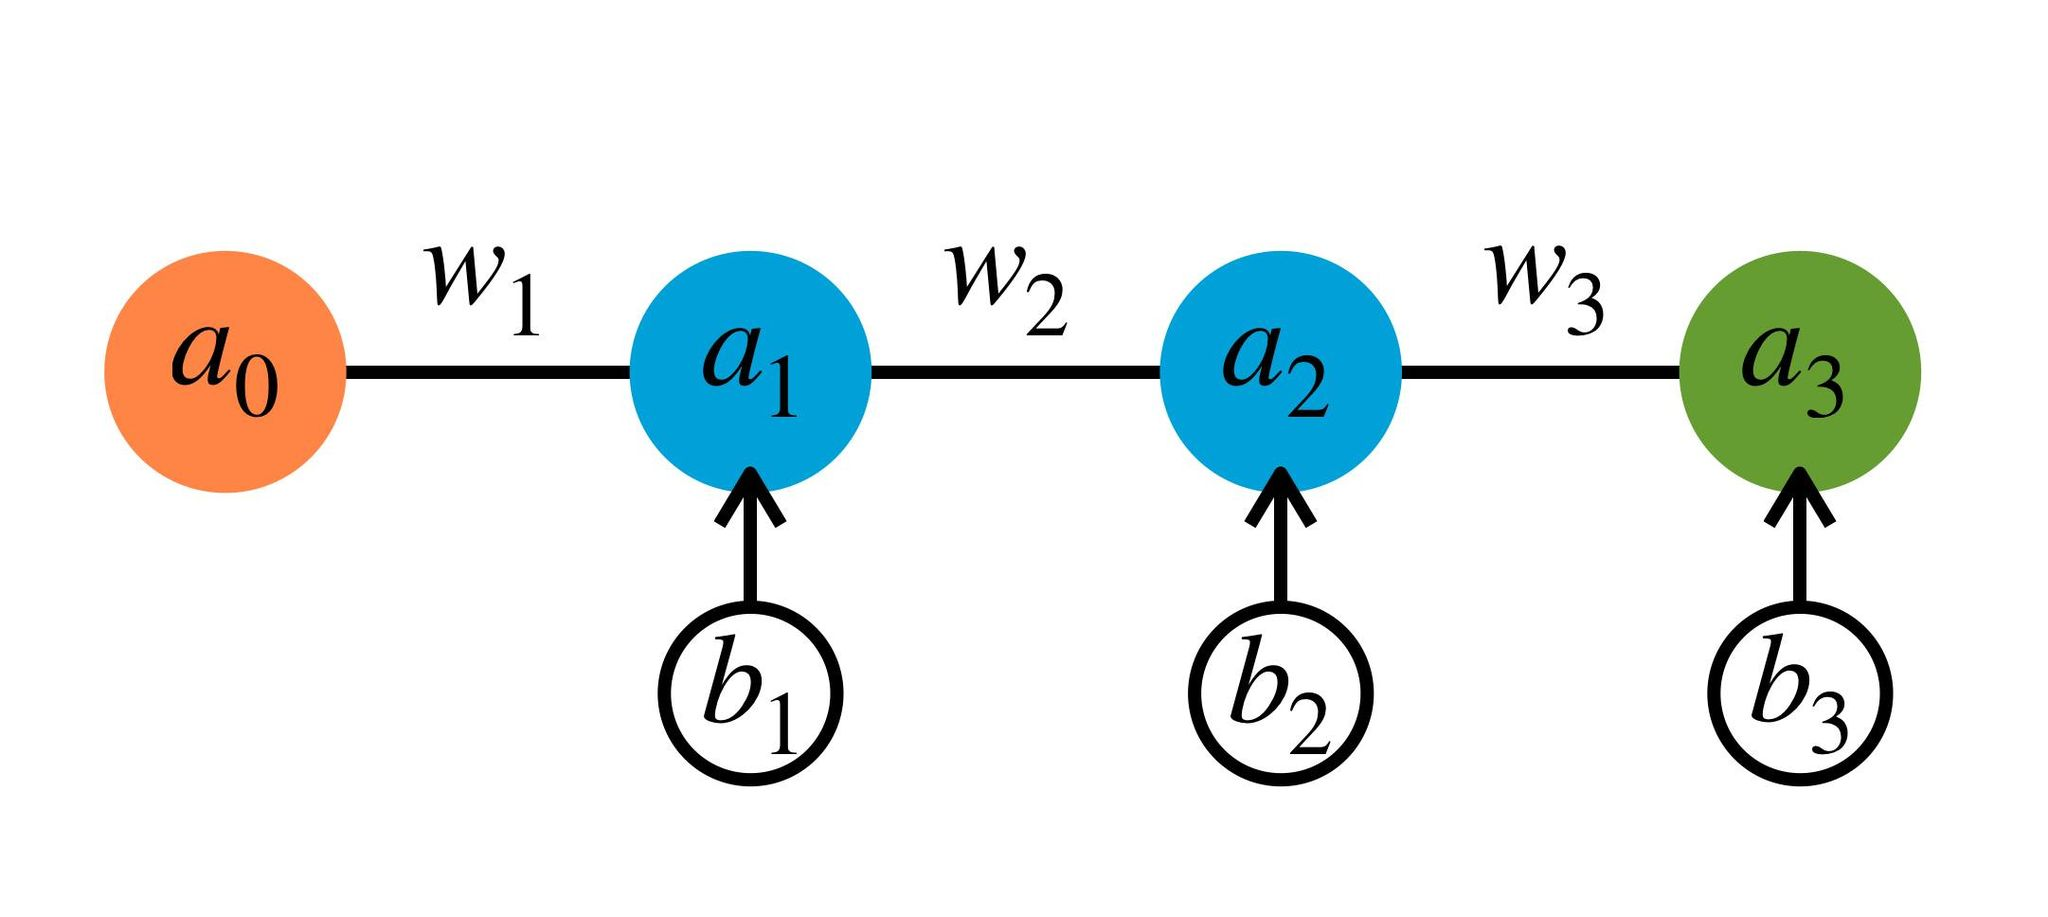
\includegraphics[width=120 mm]{images/wandb.jpg}
\caption{Minh họa mô hình mạng nơ-ron đơn giản gồm ba tầng: 1 tầng nhập (màu cam), 2 tầng ẩn (màu lam) và 1 tầng xuất (màu lục). Trong đó, $w_i$ là các trọng số liên kết, $b_i$ là hệ số bias tương ứng của từng nơ-ron và $a_i$ là giá trị kích hoạt của nơ-ron.}
\label{fig:wandb}
\end{figure}

Khi ta truyền tín hiệu đầu vào $a_0$ vào mô hình, sau khi rút trích đặc trưng qua 2 tầng ẩn, ta được kết quả dự đoán ở $a_3$. Đem so sánh kết quả tại $a_3$ với giá trị nhãn đúng $y$ ta được độ lỗi $E(\theta)$ được tính bằng công thức sau:

\begin{equation}
\begin{cases} E(\theta) = (a_3 - y)^2 \\ a_3 = \sigma(w_3\cdot a_2 + b_3) \end{cases} \\
\rightarrow E(\theta) = (\sigma(w_3\cdot a_2 + b_3) - y)^2
\end{equation}

Từ độ lỗi này, ta cần tìm đạo hàm riêng của $E(\theta)$ theo từng trọng số. Theo quy tắc mắt xích, ta có:

\begin{equation} \label{eqn:chain1}
\begin{split}
\frac{\delta E}{\delta w_3} &= \frac{\delta E}{\delta \sigma}\cdot\frac{\delta \sigma}{\delta (w_3a_2 + b_3)}\cdot \frac{\delta(w_3a_2 + b_3)}{\delta w_3} \\ &= 2(\sigma(w_3a_2+b_3)-y). \sigma(w_3a_2 + b_3)'\cdot a_2
\end{split}
\end{equation}
với $\sigma(x)$ là một hàm kích hoạt bất kỳ. Đặt $z_3 = \theta_3a_2 + b_3$, ta viết lại công thức \ref{eqn:chain1}:

\begin{equation} \label{eqn:chain2}
\frac{\delta E}{\delta w_3} = 2(\sigma(z_3)-y)\cdot \sigma(z_3)\cdot a_2
\end{equation}

Tương tự như vậy, ta có đạo hàm riêng của $E(\theta)$ tại $w_1$ và $w_2$:

\begin{equation} \label{eqn:chain3}
\begin{split}
\frac{\delta E}{\delta w_2} &= \frac{\delta E}{\delta \sigma(z_2)}\cdot\frac{\delta \sigma(z_2)}{\delta z_2}\cdot\frac{\delta z_2}{\delta w_2} \\ &= 2(\sigma(z_3)-y)\cdot \sigma(z_3)'.w_3\cdot\sigma(z_2)'\cdot a_1
\end{split}
\end{equation}
\begin{equation} \label{eqn:chain4}
\begin{split} \frac{\delta E}{\delta w_1} &= \frac{\delta E}{\delta \sigma(z_1)}\cdot\frac{\delta \sigma(z_1)}{\delta z_1}\cdot\frac{\delta z_1}{\delta w_1} \\ &= 2(\sigma(z_3)-y)\cdot \sigma(z_3)'\cdot w_3\cdot\sigma(z_2)'.w_2\cdot\sigma(z_1)'\cdot a_0
\end{split}
\end{equation}

Các công thức \ref{eqn:chain2}, \ref{eqn:chain3} và \ref{eqn:chain3} được truyền qua tập dữ liệu và lấy giá trị trung bình. Tổng hợp các giá trị này ta được véc-tơ đạo hàm riêng $\nabla_\theta \mathbf{\it{E}(\theta)}$ được dùng trong các thuật toán tối ưu khác. Tổng quát hoá cho một mô hình có $L$ tầng và số lượng nơ-ron ở mỗi tầng là $n^{(l)}$ thì độ phụ thuộc của giá trị độ lỗi vào trọng số liên kết giữa nơ-ron thứ $k$ của tầng thứ $l-1$ và nơ-ron thứ $j$ của tầng thứ $l$ là $w_{jk}$, với $z_j = ...+w_{jk}a^{l-1}_k+... + b_j$, ta có:

\begin{equation} \label{eqn:chain5}
\frac{\delta E}{\delta w_{jk}} = \frac{\delta E}{\delta \sigma(z_j)} \cdot\frac{\delta \sigma(z_j)}{\delta z_j}\cdot\frac{\delta z_j}{\delta w_{jk}}
\end{equation}
và đạo hàm riêng của độ lỗi tại nơ-ron thứ $k$ của tầng thứ $l - 1$ là giá trị tổng hợp của các hàm kích hoạt của tầng thứ $l$.

\begin{equation} \label{eqn:chain6}
\frac{\delta E}{\delta a_k^{l-1}} = \sum_{j=0}^{n^{l}-1}\frac{\delta E}{\delta \sigma(z_j)}\cdot\frac{\delta \sigma(z_j)}{\delta z_j}\cdot\frac{\delta z_j}{\delta a_k^{l-1}}
\end{equation}

Từ các công thức ta có thể nhận thấy rằng đây là quá trình cho một độ lỗi nhất định, không có công thức chung cho tất cả giá trị độ lỗi và toàn bộ quá trình sẽ phải được lặp lại khi có một độ lỗi mới. Đây là một điểm yếu của phương pháp vi phân ngược nhưng lại rất thích hợp trong huấn luyện mạng nơ-ron nhiều tầng ẩn.